\newpage

\section{Network Topology and Architecture}

This section introduces the network topology employed for the SoftEther VPN lab activity. The setup is an actual simulation where two geographically separated private networks exchange data securely across the Internet via VPN tunnels.

\subsection{GNS3 Network Simulation Platform}

The lab setup is implemented using \textbf{GNS3 (Graphical Network Simulator-3)}, a full-fledged network simulation environment that can simulate intricate virtual network topologies \cite{gns3_official}. GNS3 provides an all-in-one network learning, testing, and experimentation environment through the combination of multiple virtualization technologies into one GUI.

\noindent
\\
\textbf{Key GNS3 Features:}

GNS3 combines a range of important technologies to provide realistic network simulation:

\begin{itemize}
    \item \textbf{Router Emulation:} Supports many Routers images emulation, providing authentic router behavior and command-line interfaces
    \item \textbf{Container Integration:} Native support for Docker container enables the deployment of Linux-based network applications and services.
    \item \textbf{Virtual Machine Support:} Hypervisor support for VirtualBox and VMware to run complete operating systems
    \item \textbf{Switch Simulation:} Integrated Ethernet switching to create sophisticated network topologies
    \item \textbf{Traffic Analysis:} Integrated packet capture with Wireshark for real-time network analysis
\end{itemize}

GNS3 provides simulation of geographically sparse networks connected over Internet infrastructure, ideal in this VPN lab to learn about VPN technology without requiring several locations or sophisticated hardware setups\cite{gns3_docs}.

\subsection{Topology Overview}

The lab topology of the network consists of five major components that come together to generate a real-world Internet-based VPN scenario:

\begin{figure}[H]
\centering
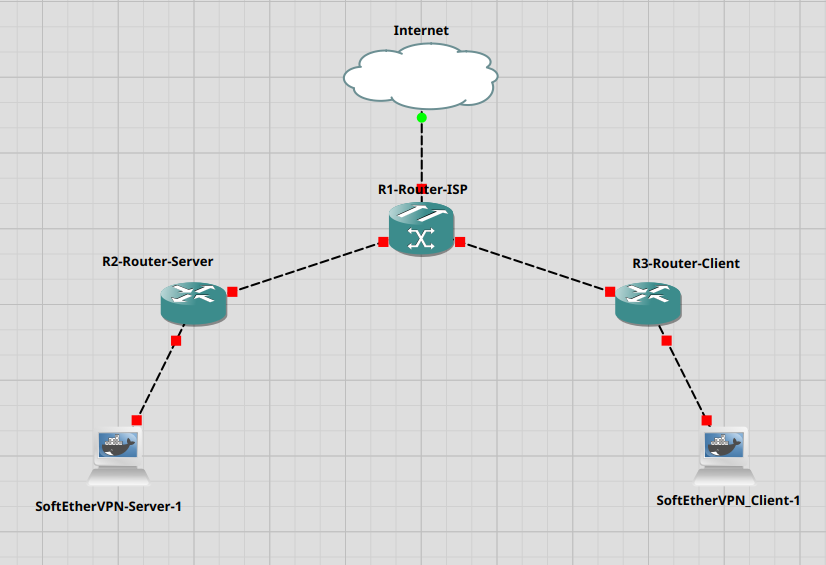
\includegraphics[width=0.8\textwidth]{../resources/Images/GNS3_Structure.png}
\caption{GNS3 Network Topology - VPN Across the Internet}
\label{fig:gns3_topology}
\end{figure}

The network topology employs an end-to-end VPN approach where:

\begin{itemize}
    \item \textbf{Server Site:} Contains the SoftEther VPN server operating within a private network
    \item \textbf{Client Site:} Represents a remote branch office that requires VPN connectivity
    \item \textbf{Internet Infrastructure:} Virtual ISP network providing public connectivity
    \item \textbf{Edge Routers:} Perform NAT and routing functions, providing Internet connectivity for the private networks
    \item \textbf{VPN Endpoints:} Docker containers hosting the actual VPN software 
\end{itemize}

This topology adequately demonstrates how end-to-end VPN technology enables secure communication between hosts of different private networks through untrusted public infrastructure, simulating common real-world deployment conditions where the VPN software runs directly on the endpoints rather than on gateway devices.

\subsection{IP Addressing Scheme}

The network address scheme uses a combination of public and private IP addresses to simulate realistic Internet connectivity. Addressing is according to RFC standards for private addressing (RFC 1918) and utilizes documentation addresses (RFC 5737) to simulate public IP.

\begin{table}[H]
\centering
\caption{Network Interface Configuration}
\label{tab:ip_addressing}
\begin{tabular}{|l|l|l|l|}
\hline
\textbf{Device} & \textbf{Interface} & \textbf{IP Address} & \textbf{Description} \\
\hline
\multirow{2}{*}{Router 2 (Server-side)} & LAN (Fa0/0) & 10.0.1.1/24 & Private Network 1 \\
 & WAN (Fa0/1) & 203.0.113.1/24 & Public IP (RFC 5737) \\
\hline
\multirow{3}{*}{ISP Router} & Interface Fa0/0 & 203.0.113.254/24 & Connected to Router 2 \\
 & Interface Fa0/1 & 198.51.100.254/24 & Connected to Router 3 \\
 & Interface Fa1/0 & DHCP Assigned & Internet Cloud \\
\hline
\multirow{2}{*}{Router 3 (Client-side)} & WAN (Fa0/1) & 198.51.100.1/24 & Public IP (RFC 5737) \\
 & LAN (Fa0/0) & 10.0.2.1/24 & Private Network 2 \\
\hline
SoftEther Server & eth0 & 10.0.1.2/24 & VPN Server Host \\
\hline
VPN Client & eth0 & 10.0.2.2/24 & VPN Client Host \\
\hline
\end{tabular}
\end{table}

\textbf{Network Segments:}

\begin{itemize}
    \item \textbf{Server Network (10.0.1.0/24):} Private subnet for hosting the SoftEther VPN server
    \item \textbf{Client Network (10.0.2.0/24):} Remote private subnet for VPN client
    \item \textbf{ISP Segment 1 (203.0.113.0/24):} Public network between ISP and server-side 
    \item \textbf{ISP Segment 2 (198.51.100.0/24):} Public network between ISP and client-side 
    \item \textbf{VPN Tunnel Networks:} Virtual addressing used for VPN connectivity (dynamically allocated)
\end{itemize}

\subsection{Device Roles and Functions}

Every device of the network topology is responsible for a particular role in demonstrating VPN functionality:

\subsubsection{ISP Router (R1-Router-ISP)}

The ISP router simulates Internet Service Provider infrastructure and provides:

\begin{itemize}
    \item \textbf{Internet Connectivity:} Public IP addressing allocated though DHCP
    \item \textbf{Inter-Site Routing:} Routes traffic among the remote sites by utilizing simulated infrastructure
    \item \textbf{NAT Traversal Support:} Enables VPN protocols to work over NAT.
    \item \textbf{Public IP Assignment:} Provides public addressing for both edge routers
\end{itemize}

The ISP router configuration contains static routes for both private networks and uses a default route towards the Internet cloud.

\subsubsection{Server-Side Router (R2-Router-Server)}

This edge router connects the private network of the server to the Internet and hosts:

\begin{itemize}
    \item \textbf{Network Address Translation:} Port Address Translation management
    \item \textbf{VPN Port Forwarding:} Static NAT rules enable forwarding of VPN traffic to the server:
        \begin{itemize}
            \item Port 500/UDP: ISAKMP forwarded to SoftEther server
            \item Port 4500/UDP: NAT-T forwarded to SoftEther server
            \item Port 443/TCP: HTTPS/TLS forwarded to SoftEther server
        \end{itemize}
    \item \textbf{Default Gateway:} Routing for the server's private network
    \item \textbf{Transparent Routing:} Routes VPN traffic between Internet and private network without VPN processing
\end{itemize}

\subsubsection{Client-Side Router (R3-Router-Client)}

The client-side edge router fulfills the same role for the remote site:

\begin{itemize}
    \item \textbf{PAT Configuration:} Network address translation for client network connectivity
    \item \textbf{Default Routing:} Internet connectivity for the client private network
    \item \textbf{Transparent VPN Support:} Allows VPN client software to connect using NAT without router-based VPN processing
\end{itemize}

\subsubsection{SoftEther VPN Server Container}

The server container runs the SoftEther VPN software with the following parameters:

\begin{itemize}
    \item \textbf{Container Image:} \texttt{siomiz/softethervpn:latest}
    \item \textbf{Multi-Protocol Support:} Concurrent IPSec and TLS/SSL VPN services
    \item \textbf{Virtual Hub:} DEFAULT hub for client connections
    \item \textbf{User Management:} Set with test user credentials for VPN authentication
    \item \textbf{Certificate Management:} Self-signed certificates for TLS-based connections
\end{itemize}

\subsubsection{VPN Client Container}

The client container simulates a remote user or branch office with:

\begin{itemize}
    \item \textbf{Container Image:} \texttt{ubuntu:latest}
    \item \textbf{IPSec Client:} StrongSwan software for IPSec connectivity
    \item \textbf{TLS Client:} OpenVPN client for SSL/TLS VPN connections
\end{itemize}

\subsection{Network Communication Flow}

The network design supports diverse communication scenarios:

\begin{enumerate}
    \item \textbf{Direct Internet Communication:} Both sites can access Internet resources through their respective ISP connections
    
    \item \textbf{End-to-End VPN Tunnel Establishment:} The VPN client container establishes direct VPN connections to the SoftEther server container using either:
    \begin{itemize}
        \item IPSec protocol (strongSwan client to SoftEther server)
        \item TLS/SSL protocol (OpenVPN client to SoftEther server)
    \end{itemize}
    
    \item \textbf{Encrypted Inter-Site Communication:} Once the VPN tunnels are created, the client will be able to communicate securely with resources in the server's network
    
    \item \textbf{NAT Traversal:} VPN protocols provide automatic NAT traversal, enabling encrypted tunnels to traverse through the edge routers
\end{enumerate}

% \subsection{Security Considerations}

% The network topology incorporates several security features:

% \begin{itemize}
%     \item \textbf{Private Addressing:} Internal networks use RFC 1918 private addresses, preventing direct Internet access
%     \item \textbf{NAT Protection:} Edge routers provide implicit firewall protection through NAT
%     \item \textbf{VPN Encryption:} All inter-site communication is protected by VPN encryption
%     \item \textbf{Authentication:} VPN connections require user credentials and/or certificates
%     \item \textbf{Protocol Separation:} Different VPN protocols operate on distinct ports for protocol isolation
% \end{itemize}

% This topology provides a foundation for comparing different VPN implementations while maintaining realistic network security practices and demonstrating practical deployment scenarios.
